\documentclass[a5paper,10pt]{booki}
\begin{document}
\begin{figure}[H]
    \centering
    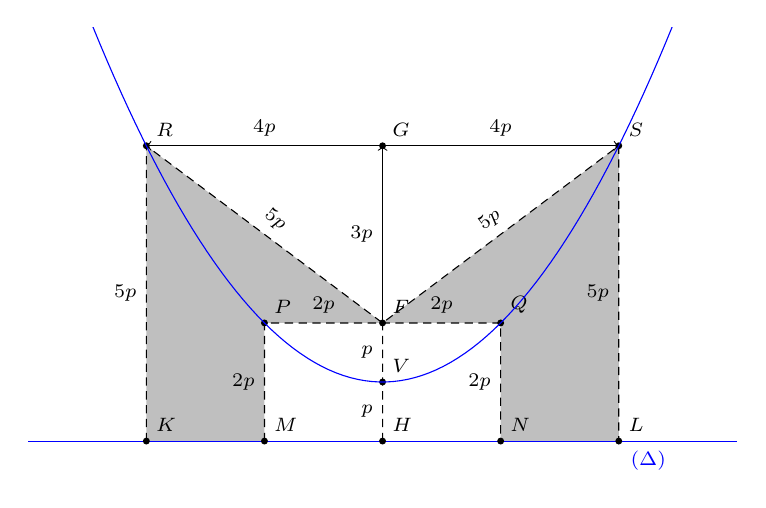
\begin{tikzpicture}[x=.75cm,y=.75cm,every node/.append style={font=\scriptsize}]
    \coordinate(D')at(-6,-1);
    \coordinate(D)at(6,-1);
    \coordinate(K)at(-4,-1);
    \coordinate(R)at(-4,4);
    \coordinate(G)at(0,4);
    \coordinate(S)at(4,4);
    \coordinate(L)at(4,-1);
    \coordinate(M)at(-2,-1);
    \coordinate(P)at(-2,1);
    \coordinate(F)at(0,1);
    \coordinate(Q)at(2,1);
    \coordinate(N)at(2,-1);
    \coordinate(V)at(0,0);
    \coordinate(H)at(0,-1);
    \fill[fill opacity=.25]
    (M)--(P)--(Q)--(N)--(L)--(S)--(F)--(R)--(K)--(M);
    \draw[color=blue](D')--node[sloped,very near end,below]{$ (\Delta) $}(D);
    \draw[->](F)--node[left]{$ 3p $}(G);
    \foreach\p in {R,S}{%
      \draw[->](G)--node[above]{$ 4p $}(\p);}
    \draw[densely dashed]
      (H)--node[left]{$ p $}(V)--node[left]{$ p $}(F)
      (M)--node[left]{$ 2p $}(P)--node[above]{$ 2p $}(F)--node[above]{$ 2p $}(Q)--node[left]{$ 2p $}(N)
      (K)--node[left]{$ 5p $}(R)--node[sloped,above]{$ 5p $}(F)--node[sloped,above]{$ 5p $}(S)--node[left]{$ 5p $}(L);
    \tkzMarkSegments[mark=s|,size=3pt](H,V V,F)
    \tkzMarkSegments[mark=s||,size=3pt](M,P P,F F,Q Q,N)
    \tkzMarkSegments[mark=o,size=2pt](K,R R,F F,S S,L)
    \foreach\p in {K,R,G,S,L,M,P,F,Q,N,V,H}{%
      \fill[color=black](\p) circle (1.25pt)node[above right]{$ \p $};}
    \clip(-6,-1) rectangle (6,6);
    \draw[color=blue,domain=-6:6,samples=100] plot(\x,{.25*\x*\x});
    \end{tikzpicture}
  \end{figure}
\end{document}